% Original pages: 49--56
% Figures: 1 unnumbered commutative diagram.
% Uncertainty log: none

so that every element of $S^{-1}A\otimes M$ is of the form $(1/s)\otimes m$. Suppose that $f((1/s)\otimes m)=0$. Then $m/s=0$, hence $tm=0$ for some $t\in S$, and therefore
\[
 \frac1s\otimes m=\frac{t}{st}\otimes m=\frac1{st}\otimes tm=\frac1{st}\otimes0=0.
\]
Hence $f$ is injective and therefore an isomorphism. \proofbox

\noindent\textit{Corollary 3.6.\amtarget{3.6} $S^{-1}A$ is a flat $A$-module.}

\noindent\textit{Proof.} \amref{3.3}, \amref{3.5}. \proofbox

\noindent\textit{Proposition 3.7.\amtarget{3.7} If $M$, $N$ are $A$-modules, there is a unique isomorphism of $S^{-1}A$-modules $f:S^{-1}M\otimes_{S^{-1}A}S^{-1}N\longrightarrow S^{-1}(M\otimes_A N)$ such that}
\[
 f((m/s)\otimes(n/t))=(m\otimes n)/st.
\]
\textit{In particular, if $\mathfrak p$ is any prime ideal, then}
\[
 M_{\mathfrak p}\otimes_{A_{\mathfrak p}}N_{\mathfrak p}\cong(M\otimes_A N)_{\mathfrak p}
\]
\textit{as $A_{\mathfrak p}$-modules.}

\noindent\textit{Proof.} Use \amref{3.5} and the canonical isomorphisms of Chapter 2. \proofbox

\subsection{Local properties}

A property $P$ of a ring $A$ (or of an $A$-module $M$) is said to be a \textit{local property} if the following is true:

$A$ (or $M$) has $P\Longleftrightarrow A_{\mathfrak p}$ (or $M_{\mathfrak p}$) has $P$, for each prime ideal $\mathfrak p$ of $A$. The following propositions give examples of local properties:

\noindent\textit{Proposition 3.8.\amtarget{3.8} Let $M$ be an $A$-module. Then the following are equivalent:}
\begin{enumerate}
\renewcommand{\labelenumi}{\roman{enumi})}
\item \textit{$M=0$;}
\item \textit{$M_{\mathfrak p}=0$ for all prime ideals $\mathfrak p$ of $A$;}
\item \textit{$M_{\mathfrak m}=0$ for all maximal ideals $\mathfrak m$ of $A$.}
\end{enumerate}

\noindent\textit{Proof.} Clearly i) $\Rightarrow$ ii) $\Rightarrow$ iii). Suppose iii) satisfied and $M\neq0$. Let $x$ be a non-zero element of $M$, and let $\mathfrak a=\operatorname{Ann}(x)$; $\mathfrak a$ is an ideal $\neq(1)$, hence is contained in a maximal ideal $\mathfrak m$ by \amref{1.4}. Consider $x/1\in M_{\mathfrak m}$. Since $M_{\mathfrak m}=0$ we have $x/1=0$, hence $x$ is killed by some element of $A-\mathfrak m$; but this is impossible since $\operatorname{Ann}(x)\subseteq\mathfrak m$. \proofbox

\noindent\textit{Proposition 3.9.\amtarget{3.9} Let $\phi:M\longrightarrow N$ be an $A$-module homomorphism. Then the following are equivalent:}
\begin{enumerate}
\renewcommand{\labelenumi}{\roman{enumi})}
\item \textit{$\phi$ is injective;}
\item \textit{$\phi_{\mathfrak p}:M_{\mathfrak p}\longrightarrow N_{\mathfrak p}$ is injective for each prime ideal $\mathfrak p$;}
\item \textit{$\phi_{\mathfrak m}:M_{\mathfrak m}\longrightarrow N_{\mathfrak m}$ is injective for each maximal ideal $\mathfrak m$.}
\end{enumerate}
\textit{Similarly with ``injective'' replaced by ``surjective'' throughout.}

\noindent\textit{Proof.} i) $\Rightarrow$ ii). $0\longrightarrow M\longrightarrow N$ is exact, hence $0\longrightarrow M_{\mathfrak p}\longrightarrow N_{\mathfrak p}$ is exact, i.e., $\phi_{\mathfrak p}$ is injective.

ii) $\Rightarrow$ iii) because a maximal ideal is prime.

iii) $\Rightarrow$ i). Let $M'=\operatorname{Ker}(\phi)$, then the sequence $0\longrightarrow M'\longrightarrow M\longrightarrow N$ is exact, hence $0\longrightarrow M'_{\mathfrak m}\longrightarrow M_{\mathfrak m}\longrightarrow N_{\mathfrak m}$ is exact by \amref{3.3} and therefore $M'_{\mathfrak m}\cong\operatorname{Ker}(\phi_{\mathfrak m})=0$ since $\phi_{\mathfrak m}$ is injective. Hence $M'=0$ by \amref{3.8}, hence $\phi$ is injective.

For the other part of the proposition, just reverse all the arrows. \proofbox

Flatness is a local property:

\noindent\textit{Proposition 3.10.\amtarget{3.10} For any $A$-module $M$, the following statements are equivalent:}
\begin{enumerate}
\renewcommand{\labelenumi}{\roman{enumi})}
\item \textit{$M$ is a flat $A$-module:}
\item \textit{$M_{\mathfrak p}$ is a flat $A_{\mathfrak p}$-module for each prime ideal $\mathfrak p$;}
\item \textit{$M_{\mathfrak m}$ is a flat $A_{\mathfrak m}$-module for each maximal ideal $\mathfrak m$.}
\end{enumerate}

\noindent\textit{Proof.} i) $\Rightarrow$ ii) by \amref{3.5} and \amref{2.20}.

ii) $\Rightarrow$ iii) O.K.

iii) $\Rightarrow$ i). If $N\longrightarrow P$ is a homomorphism of $A$-modules, and $\mathfrak m$ is any maximal ideal of $A$, then
\[
\begin{aligned}
N\longrightarrow P\text{ injective}
&\Rightarrow N_{\mathfrak m}\longrightarrow P_{\mathfrak m}\text{ injective, by \amref{3.9}}\\
&\Rightarrow N_{\mathfrak m}\otimes_{A_{\mathfrak m}}M_{\mathfrak m}\longrightarrow P_{\mathfrak m}\otimes_{A_{\mathfrak m}}M_{\mathfrak m}\text{ injective, by \amref{2.19}}\\
&\Rightarrow(N\otimes_A M)_{\mathfrak m}\longrightarrow(P\otimes_A M)_{\mathfrak m}\text{ injective, by \amref{3.7}}\\
&\Rightarrow N\otimes_A M\longrightarrow P\otimes_A M\text{ injective, by \amref{3.9}.}
\end{aligned}
\]
Hence $M$ is flat by \amref{2.19}. \proofbox

\subsection{Extended and contracted ideals in rings of fractions}

Let $A$ be a ring, $S$ a multiplicatively closed subset of $A$ and $f:A\longrightarrow S^{-1}A$ the natural homomorphism, defined by $f(a)=a/1$. Let $C$ be the set of contracted ideals in $A$, and let $E$ be the set of extended ideals in $S^{-1}A$ (cf. \amref{1.17}). If $\mathfrak a$ is an ideal in $A$, its extension $\mathfrak a^e$ in $S^{-1}A$ is $S^{-1}\mathfrak a$ (for any $y\in\mathfrak a^e$ is of the form $\sum a_i/s_i$, where $a_i\in\mathfrak a$ and $s_i\in S$; bring this fraction to a common denominator).

\noindent\textit{Proposition 3.11.\amtarget{3.11}}
\begin{enumerate}
\renewcommand{\labelenumi}{\roman{enumi})}
\item \textit{Every ideal in $S^{-1}A$ is an extended ideal.}
\item \textit{If $\mathfrak a$ is an ideal in $A$, then $\mathfrak a^{ec}=\bigcup_{s\in S}(\mathfrak a:s)$. Hence $\mathfrak a^e=(1)$ if and only if $\mathfrak a$ meets $S$.}
\item \textit{$\mathfrak a\in C\Longleftrightarrow$ no element of $S$ is a zero-divisor in $A/\mathfrak a$.}
\item \textit{The prime ideals of $S^{-1}A$ are in one-to-one correspondence ($\mathfrak p\longleftrightarrow S^{-1}\mathfrak p$) with the prime ideals of $A$ which don't meet $S$.}
\item \textit{The operation $S^{-1}$ commutes with formation of finite sums, products, intersections and radicals.}
\end{enumerate}

\noindent\textit{Proof.} i) Let $\mathfrak b$ be an ideal in $S^{-1}A$, and let $x/s\in\mathfrak b$. Then $x/1\in\mathfrak b$, hence $x\in\mathfrak b^c$ and therefore $x/s\in\mathfrak b^{ce}$. Since $\mathfrak b\supseteq\mathfrak b^{ce}$ in any case \amref{1.17}, it follows that $\mathfrak b=\mathfrak b^{ce}$.

ii) $x\in\mathfrak a^{ec}=(S^{-1}\mathfrak a)^c\Longleftrightarrow x/1=a/s$ for some $a\in\mathfrak a$, $s\in S\Longleftrightarrow(xs-a)t=0$ for some $t\in S\Longleftrightarrow xst\in\mathfrak a\Longleftrightarrow x\in\bigcup_{s\in S}(\mathfrak a:s)$.

iii) $\mathfrak a\in C\Longleftrightarrow\mathfrak a^{ec}\subseteq\mathfrak a\Longleftrightarrow(sx\in\mathfrak a$ for some $s\in S\Rightarrow x\in\mathfrak a)\Longleftrightarrow$ no $s\in S$ is a zero-divisor in $A/\mathfrak a$.

iv) If $\mathfrak q$ is a prime ideal in $S^{-1}A$, then $\mathfrak q^c$ is a prime ideal in $A$ (this much is true for any ring homomorphism). Conversely, if $\mathfrak p$ is a prime ideal in $A$, then $A/\mathfrak p$ is an integral domain; if $\overline S$ is the image of $S$ in $A/\mathfrak p$, we have $S^{-1}A/S^{-1}\mathfrak p\cong\overline S^{-1}(A/\mathfrak p)$ which is either $0$ or else is contained in the field of fractions of $A/\mathfrak p$ and is therefore an integral domain, and therefore $S^{-1}\mathfrak p$ is either prime or is the unit ideal; by i) the latter possibility occurs if and only if $\mathfrak p$ meets $S$.

v) For sums and products, this follows from \amref{1.18}; for intersections, from \amref{3.4}. As to radicals, we have $S^{-1}r(\mathfrak a)\subseteq r(S^{-1}\mathfrak a)$ from \amref{1.18}, and the proof of the reverse inclusion is a routine verification which we leave to the reader. \proofbox

\noindent\textit{Remarks.} 1) If $\mathfrak a$, $\mathfrak b$ are ideals of $A$, the formula
\[
 S^{-1}(\mathfrak a:\mathfrak b)=(S^{-1}\mathfrak a:S^{-1}\mathfrak b)
\]
is true provided the ideal $\mathfrak b$ is finitely generated: see \amref{3.15}.

2) The proof in \amref{1.8} that if $f\in A$ is not nilpotent there is a prime ideal of $A$ which does not contain $f$ can be expressed more concisely in the language of rings of fractions. Since the set $S=(f^n)_{n\geq0}$ does not contain $0$, the ring $S^{-1}A=A_f$ is not the zero ring and therefore by \amref{1.3} has a maximal ideal, whose contraction in $A$ is a prime ideal $\mathfrak p$ which does not meet $S$ by \amref{3.11}; hence $f\notin\mathfrak p$.

\noindent\textit{Corollary 3.12.\amtarget{3.12} If $\mathfrak N$ is the nilradical of $A$, the nilradical of $S^{-1}A$ is $S^{-1}\mathfrak N$.} \proofbox

\noindent\textit{Corollary 3.13.\amtarget{3.13} If $\mathfrak p$ is a prime ideal of $A$, the prime ideals of the local ring $A_{\mathfrak p}$ are in one-to-one correspondence with the prime ideals of $A$ contained in $\mathfrak p$.}

\noindent\textit{Proof.} Take $S=A-\mathfrak p$ in \amref{3.11} (iv). \proofbox

\noindent\textit{Remark.} Thus the passage from $A$ to $A_{\mathfrak p}$ cuts out all prime ideals except those contained in $\mathfrak p$. In the other direction, the passage from $A$ to $A/\mathfrak p$ cuts out all prime ideals except those containing $\mathfrak p$. Hence if $\mathfrak p$, $\mathfrak q$ are prime ideals such that $\mathfrak p\supseteq\mathfrak q$, then by localizing with respect to $\mathfrak p$ and taking the quotient mod $\mathfrak q$ (in either order: these two operations commute, by \amref{3.4}), we restrict our attention to those prime ideals which lie between $\mathfrak p$ and $\mathfrak q$. In particular, if $\mathfrak p=\mathfrak q$ we end up with a field, called the \textit{residue field at $\mathfrak p$}, which can be obtained either as the field of fractions of the integral domain $A/\mathfrak p$ or as the residue field of the local ring $A_{\mathfrak p}$.

\noindent\textit{Proposition 3.14.\amtarget{3.14} Let $M$ be a finitely generated $A$-module, $S$ a multiplicatively closed subset of $A$. Then $S^{-1}(\operatorname{Ann}(M))=\operatorname{Ann}(S^{-1}M)$.}

\noindent\textit{Proof.} If this is true for two $A$-modules, $M$, $N$, it is true for $M+N$:
\[
\begin{aligned}
S^{-1}(\operatorname{Ann}(M+N))
&=S^{-1}(\operatorname{Ann}(M)\cap\operatorname{Ann}(N)) &&\text{by \amref{2.2}}\\
&=S^{-1}(\operatorname{Ann}(M))\cap S^{-1}(\operatorname{Ann}(N)) &&\text{by \amref{3.4}}\\
&=\operatorname{Ann}(S^{-1}M)\cap\operatorname{Ann}(S^{-1}N) &&\text{by hypothesis}\\
&=\operatorname{Ann}(S^{-1}M+S^{-1}N)=\operatorname{Ann}(S^{-1}(M+N)).
\end{aligned}
\]
Hence it is enough to prove \amref{3.14} for $M$ generated by a single element: then $M\cong A/\mathfrak a$ (as $A$-module), where $\mathfrak a=\operatorname{Ann}(M)$; $S^{-1}M\cong(S^{-1}A)/(S^{-1}\mathfrak a)$ by \amref{3.4}, so that $\operatorname{Ann}(S^{-1}M)=S^{-1}\mathfrak a=S^{-1}(\operatorname{Ann}(M))$. \proofbox

\noindent\textit{Corollary 3.15.\amtarget{3.15} If $N$, $P$ are submodules of an $A$-module $M$ and if $P$ is finitely generated, then $S^{-1}(N:P)=(S^{-1}N:S^{-1}P)$.}

\noindent\textit{Proof.} $(N:P)=\operatorname{Ann}((N+P)/N)$ by \amref{2.2}; now apply \amref{3.14}. \proofbox

\noindent\textit{Proposition 3.16.\amtarget{3.16} Let $A\longrightarrow B$ be a ring homomorphism and let $\mathfrak p$ be a prime ideal of $A$. Then $\mathfrak p$ is the contraction of a prime ideal of $B$ if and only if $\mathfrak p^{ec}=\mathfrak p$.}

\noindent\textit{Proof.} If $\mathfrak p=\mathfrak q^c$ then $\mathfrak p^{ec}=\mathfrak p$ by \amref{1.17}. Conversely, if $\mathfrak p^{ec}=\mathfrak p$, let $S$ be the image of $A-\mathfrak p$ in $B$. Then $\mathfrak p^e$ does not meet $S$, therefore by \amref{3.11} its extension in $S^{-1}B$ is a proper ideal and hence is contained in a maximal ideal $\mathfrak m$ of $S^{-1}B$. If $\mathfrak q$ is the contraction of $\mathfrak m$ in $B$, then $\mathfrak q$ is prime, $\mathfrak q\supseteq\mathfrak p^e$ and $\mathfrak q\cap S=\varnothing$. Hence $\mathfrak q^c=\mathfrak p$. \proofbox

\subsection{Exercises}

\begin{enumerate}
\item Let $S$ be a multiplicatively closed subset of a ring $A$, and let $M$ be a finitely generated $A$-module. Prove that $S^{-1}M=0$ if and only if there exists $s\in S$ such that $sM=0$.

\item Let $\mathfrak a$ be an ideal of a ring $A$, and let $S=1+\mathfrak a$. Show that $S^{-1}\mathfrak a$ is contained in the Jacobson radical of $S^{-1}A$.

Use this result and Nakayama's lemma to give a proof of \amref{2.5} which does not depend on determinants. [If $M=\mathfrak aM$, then $S^{-1}M=(S^{-1}\mathfrak a)(S^{-1}M)$, hence by Nakayama we have $S^{-1}M=0$. Now use Exercise 1.]

\item Let $A$ be a ring, let $S$ and $T$ be two multiplicatively closed subsets of $A$, and let $U$ be the image of $T$ in $S^{-1}A$. Show that the rings $(ST)^{-1}A$ and $U^{-1}(S^{-1}A)$ are isomorphic.

\item Let $f:A\longrightarrow B$ be a homomorphism of rings and let $S$ be a multiplicatively closed subset of $A$. Let $T=f(S)$. Show that $S^{-1}B$ and $T^{-1}B$ are isomorphic as $S^{-1}A$-modules.

\item Let $A$ be a ring. Suppose that, for each prime ideal $\mathfrak p$, the local ring $A_{\mathfrak p}$ has no nilpotent element $\neq0$. Show that $A$ has no nilpotent element $\neq0$. If each $A_{\mathfrak p}$ is an integral domain, is $A$ necessarily an integral domain?

\item Let $A$ be a ring $\neq0$ and let $\Sigma$ be the set of all multiplicatively closed subsets $S$ of $A$ such that $0\notin S$. Show that $\Sigma$ has maximal elements, and that $S\in\Sigma$ is maximal if and only if $A-S$ is a minimal prime ideal of $A$.

\item A multiplicatively closed subset $S$ of a ring $A$ is said to be \textit{saturated} if
\[
 xy\in S\Longleftrightarrow x\in S\text{ and }y\in S.
\]
Prove that
\begin{enumerate}
\renewcommand{\labelenumii}{\roman{enumii})}
\item $S$ is saturated $\Longleftrightarrow A-S$ is a union of prime ideals.
\item If $S$ is any multiplicatively closed subset of $A$, there is a unique smallest saturated multiplicatively closed subset $\overline S$ containing $S$, and that $\overline S$ is the complement in $A$ of the union of the prime ideals which do not meet $S$. ($\overline S$ is called the \textit{saturation} of $S$.)
\end{enumerate}
If $S=1+\mathfrak a$, where $\mathfrak a$ is an ideal of $A$, find $\overline S$.

\item Let $S$, $T$ be multiplicatively closed subsets of $A$, such that $S\subseteq T$. Let $\phi:S^{-1}A\longrightarrow T^{-1}A$ be the homomorphism which maps each $a/s\in S^{-1}A$ to $a/s$ considered as an element of $T^{-1}A$. Show that the following statements are equivalent:
\begin{enumerate}
\renewcommand{\labelenumii}{\roman{enumii})}
\item $\phi$ is bijective.
\item For each $t\in T$, $t/1$ is a unit in $S^{-1}A$.
\item For each $t\in T$ there exists $x\in A$ such that $xt\in S$.
\item $T$ is contained in the saturation of $S$ (Exercise 7).
\item Every prime ideal which meets $T$ also meets $S$.
\end{enumerate}

\item The set $S_0$ of all non-zero-divisors in $A$ is a saturated multiplicatively closed subset of $A$. Hence the set $D$ of zero-divisors in $A$ is a union of prime ideals (see Chapter 1, Exercise 14). Show that every minimal prime ideal of $A$ is contained in $D$. [Use Exercise 6.]

The ring $S_0^{-1}A$ is called the \textit{total ring of fractions} of $A$. Prove that
\begin{enumerate}
\renewcommand{\labelenumii}{\roman{enumii})}
\item $S_0$ is the largest multiplicatively closed subset of $A$ for which the homomorphism $A\longrightarrow S_0^{-1}A$ is injective.
\item Every element in $S_0^{-1}A$ is either a zero-divisor or a unit.
\item Every ring in which every non-unit is a zero-divisor is equal to its total ring of fractions (i.e., $A\longrightarrow S_0^{-1}A$ is bijective).
\end{enumerate}

\item Let $A$ be a ring.
\begin{enumerate}
\renewcommand{\labelenumii}{\roman{enumii})}
\item If $A$ is absolutely flat (Chapter 2, Exercise 27) and $S$ is any multiplicatively closed subset of $A$, then $S^{-1}A$ is absolutely flat.
\item $A$ is absolutely flat $\Longleftrightarrow A_{\mathfrak m}$ is a field for each maximal ideal $\mathfrak m$.
\end{enumerate}

\item Let $A$ be a ring. Prove that the following are equivalent:
\begin{enumerate}
\renewcommand{\labelenumii}{\roman{enumii})}
\item $A/\mathfrak N$ is absolutely flat ($\mathfrak N$ being the nilradical of $A$).
\item Every prime ideal of $A$ is maximal.
\item $\operatorname{Spec}(A)$ is a $T_1$-space (i.e., every subset consisting of a single point is closed).
\item $\operatorname{Spec}(A)$ is Hausdorff.
\end{enumerate}
If these conditions are satisfied, show that $\operatorname{Spec}(A)$ is compact and totally disconnected (i.e. the only connected subsets of $\operatorname{Spec}(A)$ are those consisting of a single point).

\item Let $A$ be an integral domain and $M$ an $A$-module. An element $x\in M$ is a \textit{torsion element} of $M$ if $\operatorname{Ann}(x)\neq0$, that is if $x$ is killed by some non-zero element of $A$. Show that the torsion elements of $M$ form a submodule of $M$. This submodule is called the \textit{torsion submodule} of $M$ and is denoted by $T(M)$. If $T(M)=0$, the module $M$ is said to be torsion-free. Show that
\begin{enumerate}
\renewcommand{\labelenumii}{\roman{enumii})}
\item If $M$ is any $A$-module, then $M/T(M)$ is torsion-free.
\item If $f:M\longrightarrow N$ is a module homomorphism, then $f(T(M))\subseteq T(N)$.
\item If $0\longrightarrow M'\longrightarrow M\longrightarrow M''$ is an exact sequence, then the sequence $0\longrightarrow T(M')\longrightarrow T(M)\longrightarrow T(M'')$ is exact.
\item If $M$ is any $A$-module, then $T(M)$ is the kernel of the mapping $x\mapsto1\otimes x$ of $M$ into $K\otimes_A M$, where $K$ is the field of fractions of $A$.
\end{enumerate}
[For iv), show that $K$ may be regarded as the direct limit of its submodules $A\xi$ ($\xi\in K$); using Chapter 1, Exercise 15 and Exercise 20, show that if $1\otimes x=0$ in $K\otimes M$ then $1\otimes x=0$ in $A\xi\otimes M$ for some $\xi\neq0$. Deduce that $\xi^{-1}x=0$.]

\item Let $S$ be a multiplicatively closed subset of an integral domain $A$. In the notation of Exercise 12, show that $T(S^{-1}M)=S^{-1}(T(M))$. Deduce that the following are equivalent:
\begin{enumerate}
\renewcommand{\labelenumii}{\roman{enumii})}
\item $M$ is torsion-free.
\item $M_{\mathfrak p}$ is torsion-free for all prime ideals $\mathfrak p$.
\item $M_{\mathfrak m}$ is torsion-free for all maximal ideals $\mathfrak m$.
\end{enumerate}

\item Let $M$ be an $A$-module and $\mathfrak a$ an ideal of $A$. Suppose that $M_{\mathfrak m}=0$ for all maximal ideals $\mathfrak m\supseteq\mathfrak a$. Prove that $M=\mathfrak aM$. [Pass to the $A/\mathfrak a$-module $M/\mathfrak aM$ and use \amref{3.8}.]

\item Let $A$ be a ring, and let $F$ be the $A$-module $A^n$. Show that every set of $n$ generators of $F$ is a basis of $F$. [Let $x_1,\ldots,x_n$ be a set of generators and $e_1,\ldots,e_n$ the canonical basis of $F$. Define $\phi:F\longrightarrow F$ by $\phi(e_i)=x_i$. Then $\phi$ is surjective and we have to prove that it is an isomorphism. By \amref{3.9} we may assume that $A$ is a local ring. Let $N$ be the kernel of $\phi$ and let $k=A/\mathfrak m$ be the residue field of $A$. Since $F$ is a flat $A$-module, the exact sequence $0\longrightarrow N\longrightarrow F\longrightarrow F\longrightarrow0$ gives an exact sequence
\[
 0\longrightarrow k\otimes N\longrightarrow k\otimes F\xrightarrow{1\otimes\phi}k\otimes F\longrightarrow0.
\]
Now $k\otimes F=k^n$ is an $n$-dimensional vector space over $k$; $1\otimes\phi$ is surjective, hence bijective, hence $k\otimes N=0$.

Also $N$ is finitely generated, by Chapter 2, Exercise 12, hence $N=0$ by Nakayama's lemma. Hence $\phi$ is an isomorphism.]

Deduce that every set of generators of $F$ has at least $n$ elements.

\item Let $B$ be a flat $A$-algebra. Then the following conditions are equivalent:
\begin{enumerate}
\renewcommand{\labelenumii}{\roman{enumii})}
\item $\mathfrak a^{ec}=\mathfrak a$ for all ideals $\mathfrak a$ of $A$.
\item $\operatorname{Spec}(B)\longrightarrow\operatorname{Spec}(A)$ is surjective.
\item For every maximal ideal $\mathfrak m$ of $A$ we have $\mathfrak m^e\neq(1)$.
\item If $M$ is any non-zero $A$-module, then $M_B\neq0$.
\item For every $A$-module $M$, the mapping $x\mapsto1\otimes x$ of $M$ into $M_B$ is injective.
\end{enumerate}
[For i) $\Rightarrow$ ii), use \amref{3.16}. ii) $\Rightarrow$ iii) is clear.

iii) $\Rightarrow$ iv): Let $x$ be a non-zero element of $M$ and let $M'=Ax$. Since $B$ is flat over $A$ it is enough to show that $M_B'\neq0$. We have $M'\cong A/\mathfrak a$ for some ideal $\mathfrak a\neq(1)$, hence $M_B'\cong B/\mathfrak a^e$. Now $\mathfrak a\subseteq\mathfrak m$ for some maximal ideal $\mathfrak m$, hence $\mathfrak a^e\subseteq\mathfrak m^e\neq(1)$. Hence $M_B'\neq0$.

iv) $\Rightarrow$ v): Let $M'$ be the kernel of $M\longrightarrow M_B$. Since $B$ is flat over $A$, the sequence $0\longrightarrow M_B'\longrightarrow M_B\longrightarrow(M_B)_B$ is exact. But (Chapter 2, Exercise 13, with $N=M_B$) the mapping $M_B\longrightarrow(M_B)_B$ is injective, hence $M_B'=0$ and therefore $M'=0$.

v) $\Rightarrow$ i): Take $M=A/\mathfrak a$.]

$B$ is said to be \textit{faithfully flat} over $A$.

\item Let $A\xrightarrow{f}B\xrightarrow{g}C$ be ring homomorphisms. If $g\circ f$ is flat and $g$ is faithfully flat, then $f$ is flat.

\item Let $f:A\longrightarrow B$ be a flat homomorphism of rings, let $\mathfrak q$ be a prime ideal of $B$ and let $\mathfrak p=\mathfrak q^c$. Then $f^*:\operatorname{Spec}(B_{\mathfrak q})\longrightarrow\operatorname{Spec}(A_{\mathfrak p})$ is surjective. [For $B_{\mathfrak p}$ is flat over $A_{\mathfrak p}$ by \amref{3.10}, and $B_{\mathfrak q}$ is a local ring of $B_{\mathfrak p}$, hence is flat over $B_{\mathfrak p}$. Hence $B_{\mathfrak q}$ is flat over $A_{\mathfrak p}$ and satisfies condition (3) of Exercise 16.]

\item Let $A$ be a ring, $M$ an $A$-module. The \textit{support} of $M$ is defined to be the set $\operatorname{Supp}(M)$ of prime ideals $\mathfrak p$ of $A$ such that $M_{\mathfrak p}\neq0$. Prove the following results:
\begin{enumerate}
\renewcommand{\labelenumii}{\roman{enumii})}
\item $M\neq0\Longleftrightarrow\operatorname{Supp}(M)\neq\varnothing$.
\item $V(\mathfrak a)=\operatorname{Supp}(A/\mathfrak a)$.
\item If $0\longrightarrow M'\longrightarrow M\longrightarrow M''\longrightarrow0$ is an exact sequence, then $\operatorname{Supp}(M)=\operatorname{Supp}(M')\cup\operatorname{Supp}(M'')$.
\item If $M=\sum M_i$, then $\operatorname{Supp}(M)=\bigcup\operatorname{Supp}(M_i)$.
\item If $M$ is finitely generated, then $\operatorname{Supp}(M)=V(\operatorname{Ann}(M))$ (and is therefore a closed subset of $\operatorname{Spec}(A)$).
\item If $M$, $N$ are finitely generated, then $\operatorname{Supp}(M\otimes_A N)=\operatorname{Supp}(M)\cap\operatorname{Supp}(N)$. [Use Chapter 2, Exercise 3.]
\item If $M$ is finitely generated and $\mathfrak a$ is an ideal of $A$, then $\operatorname{Supp}(M/\mathfrak aM)=V(\mathfrak a+\operatorname{Ann}(M))$.
\item If $f:A\longrightarrow B$ is a ring homomorphism and $M$ is a finitely generated $A$-module, then $\operatorname{Supp}(B\otimes_A M)=f^{*-1}(\operatorname{Supp}(M))$.
\end{enumerate}

\item Let $f:A\longrightarrow B$ be a ring homomorphism, $f^*:\operatorname{Spec}(B)\longrightarrow\operatorname{Spec}(A)$ the associated mapping. Show that
\begin{enumerate}
\renewcommand{\labelenumii}{\roman{enumii})}
\item Every prime ideal of $A$ is a contracted ideal $\Longleftrightarrow f^*$ is surjective.
\item Every prime ideal of $B$ is an extended ideal $\Rightarrow f^*$ is injective.
\end{enumerate}
Is the converse of ii) true?

\item
\begin{enumerate}
\renewcommand{\labelenumii}{\roman{enumii})}
\item Let $A$ be a ring, $S$ a multiplicatively closed subset of $A$, and $\phi:A\longrightarrow S^{-1}A$ the canonical homomorphism. Show that $\phi^*:\operatorname{Spec}(S^{-1}A)\longrightarrow\operatorname{Spec}(A)$ is a homeomorphism of $\operatorname{Spec}(S^{-1}A)$ onto its image in $X=\operatorname{Spec}(A)$. Let this image be denoted by $S^{-1}X$.

In particular, if $f\in A$, the image of $\operatorname{Spec}(A_f)$ in $X$ is the basic open set $X_f$ (Chapter 1, Exercise 17).

\item Let $f:A\longrightarrow B$ be a ring homomorphism. Let $X=\operatorname{Spec}(A)$ and $Y=\operatorname{Spec}(B)$, and let $f^*:Y\longrightarrow X$ be the mapping associated with $f$. Identifying $\operatorname{Spec}(S^{-1}A)$ with its canonical image $S^{-1}X$ in $X$, and $\operatorname{Spec}(S^{-1}B)$ ($=\operatorname{Spec}(f(S)^{-1}B)$) with its canonical image $S^{-1}Y$ in $Y$, show that $S^{-1}f^*:\operatorname{Spec}(S^{-1}B)\longrightarrow\operatorname{Spec}(S^{-1}A)$ is the restriction of $f^*$ to $S^{-1}Y$, and that $S^{-1}Y=f^{*-1}(S^{-1}X)$.

\item Let $\mathfrak a$ be an ideal of $A$ and let $\mathfrak b=\mathfrak a^e$ be its extension in $B$. Let $\bar f:A/\mathfrak a\longrightarrow B/\mathfrak b$ be the homomorphism induced by $f$. If $\operatorname{Spec}(A/\mathfrak a)$ is identified with its canonical image $V(\mathfrak a)$ in $X$, and $\operatorname{Spec}(B/\mathfrak b)$ with its image $V(\mathfrak b)$ in $Y$, show that $\bar f^*$ is the restriction of $f^*$ to $V(\mathfrak b)$.

\item Let $\mathfrak p$ be a prime ideal of $A$. Take $S=A-\mathfrak p$ in ii) and then reduce mod $S^{-1}\mathfrak p$ as in iii). Deduce that the subspace $f^{*-1}(\mathfrak p)$ of $Y$ is naturally homeomorphic to $\operatorname{Spec}(B_{\mathfrak p}/\mathfrak pB_{\mathfrak p})=\operatorname{Spec}(k(\mathfrak p)\otimes_A B)$, where $k(\mathfrak p)$ is the residue field of the local ring $A_{\mathfrak p}$.

$\operatorname{Spec}(k(\mathfrak p)\otimes_A B)$ is called the \textit{fiber} of $f^*$ over $\mathfrak p$.
\end{enumerate}

\item Let $A$ be a ring and $\mathfrak p$ a prime ideal of $A$. Then the canonical image of $\operatorname{Spec}(A_{\mathfrak p})$ in $\operatorname{Spec}(A)$ is equal to the intersection of all the open neighborhoods of $\mathfrak p$ in $\operatorname{Spec}(A)$.

\item Let $A$ be a ring, let $X=\operatorname{Spec}(A)$ and let $U$ be a basic open set in $X$ (i.e., $U=X_f$ for some $f\in A$: Chapter 1, Exercise 17).
\begin{enumerate}
\renewcommand{\labelenumii}{\roman{enumii})}
\item If $U=X_f$, show that the ring $A(U)=A_f$ depends only on $U$ and not on $f$.
\item Let $U'=X_g$ be another basic open set such that $U'\subseteq U$. Show that there is an equation of the form $g^n=uf$ for some integer $n>0$ and some $u\in A$, and use this to define a homomorphism $\rho:A(U)\longrightarrow A(U')$ (i.e., $A_f\longrightarrow A_g$) by mapping $a/f^m$ to $au^m/g^{mn}$. Show that $\rho$ depends only on $U$ and $U'$. This homomorphism is called the \textit{restriction homomorphism}.
\item If $U=U'$, then $\rho$ is the identity map.
\item If $U\supseteq U'\supseteq U''$ are basic open sets in $X$, show that the diagram

\begin{center}
% Unnumbered restriction-homomorphism diagram from original page 56.
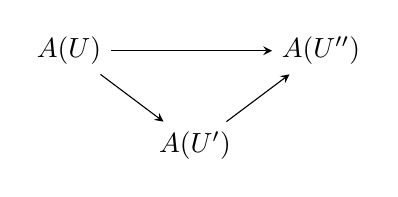
\begin{tikzpicture}[baseline=(current bounding box.center),>=stealth]
  \node (AU) at (0,1.2) {$A(U)$};
  \node (AUpp) at (3.2,1.2) {$A(U'')$};
  \node (AUp) at (1.6,0) {$A(U')$};

  \draw[->] (AU) -- (AUpp);
  \draw[->] (AU) -- (AUp);
  \draw[->] (AUp) -- (AUpp);
\end{tikzpicture}

\end{center}

(in which the arrows are restriction homomorphisms) is commutative.
\item Let $x$ ($=\mathfrak p$) be a point of $X$. Show that
\[
 \varinjlim_{U\ni x}A(U)\cong A_{\mathfrak p}.
\]
\end{enumerate}

The assignment of the ring $A(U)$ to each basic open set $U$ of $X$, and the restriction homomorphisms $\rho$, satisfying the conditions iii) and iv) above, constitutes a \textit{presheaf of rings} on the basis of open sets $(X_f)_{f\in A}$. v) says that the stalk of this presheaf at $x\in X$ is the corresponding local ring $A_{\mathfrak p}$.

\item Show that the presheaf of Exercise 23 has the following property. Let $(U_i)_{i\in I}$ be a covering of $X$ by basic open sets. For each $i\in I$ let $s_i\in A(U_i)$ be such that, for each pair of indices $i,j$, the images of $s_i$ and $s_j$ in $A(U_i\cap U_j)$ are equal. Then there exists a unique $s\in A$ ($=A(X)$) whose image in $A(U_i)$ is $s_i$, for all $i\in I$. (This essentially implies that the presheaf is a sheaf.)
\end{enumerate}
